\section{Data Analysis}
\label{sec:Analysis}
\subsection{Analysis Strategy}
\begin{table}[b]
\centering{
\begin{tabular}{@{} rcl @{}}
  \toprule
  Particle & Decay Mode & Branching Ratio \\ \midrule
  $a_1$ & \qquad \qquad \qquad \qquad $\pi^{0}\gamma$ \qquad \qquad \qquad \qquad & $(0.15 \pm 0.07)$\% \\ 
  $a_1$ & \qquad \qquad $\pi^0\pi^{+}\pi^{-}$ \qquad \qquad & seen, BR not known\\ \midrule
  $\omega$ & \qquad \qquad $\pi^{0}\gamma$ \qquad \qquad & $(8.40 \pm 0.22)$\% \\
  $\omega$ & \qquad \qquad $\pi^0\pi^{+}\pi^{-}$ \qquad \qquad & $(89.3 \pm 0.06)$\% \\ \midrule
  $\eta$ & \qquad \qquad $\pi^0\pi^{+}\pi^{-}$ \qquad \qquad & $(22.92 \pm 0.28)$\% \\ \midrule
  $\rho$ & \qquad \qquad $\pi^{+}\pi^{-}$ \qquad \qquad & $\sim 100$\% \\
  \bottomrule 
\end{tabular}
}
\caption{Decay modes of the $a_1$ meson and control modes $\omega,\eta$ and $\rho$ \cite{PDG2018}}
\label{tab:pdg}
\end{table}
In the first section, we got a first insight on the importance of the $a_1$-$\rho$ system as a probe for chiral symmetry restoration. Eventually, one would like to measure the $a_1$ in heavy-ion collisions decaying only into electromagnetically interacting particles so effects of the QGP would be visible. Since this is a feasibility study of the measurement of the $a_1$ in the ALICE detector we use the decay modes which can be most easily tracked with the detector. With its TPC the ALICE detector has a very precise tool to trace charged particles. The ALICE detector also offers three calorimeters, the PHOS, the EMCAL and the DCAL which can be used to measure the energy of neutral particles. Looking at table \ref{tab:pdg} what we want to do to analyse the $a_1$ in the $\pi^0 \gamma$ channel, is to hope for the neutral pion to decay into two photons (which happens in approximately 99\% of the cases \cite{PDG2018}) and then measure them along with the other photon from the $a_1$ decay with the calorimeters. The other option is two hope for all of the photons to decay in the detector material and then use the dielectron pairs from the conversion to reconstruct the $a_1$. For the $\pi^0 \pi^{+}\pi^{-}$ decay channel we can use the tracking capabilities of the TPC to trace the charged pions and then do the same procedure as for the other decay channel for the neutral pion. \\
Both techniques obviously have their advantages and disadvantages. The photon conversion method (PCM) works very well at low transverse momenta. This is because it uses the tracks of the charged particles to reconstruct the photon. Obviously the track of a particle with lower momentum will be bent more, i.e. have a smaller radius of curvature, then a particle with high momentum. Therefore a smaller radius of curvature should mean a better, i.e. smaller, resolution. We can estimate a resolution with $\sigma_{PCM} \sim R = \frac{p_T}{qB}$ by setting the centrifugal force of a particle equal to the Lorentz force in a magnetic field and assuming $p \simeq p_T$. For constant magnetic field and charge this estimate of the resolution obviously gets better with lower $p_T$. Another advantage is that particles can be identified relatively easily, e.g. using their specific energy loss in the TPC. One of the biggest disadvantages of PCM is the conversion probability. The conversion probability for ALICE for the integrated detector material for $R<180$ cm and $|\eta|<0.9$ is about 8.5\% \cite{ALICEPerfRep}. If we then have to take this to the power of three for the $\pi^0\gamma$ channel, this really dampens the already low probability to find the $a_1$ even more. \\
For the calorimeters we can also make a quick approximation of the resolution. If we assume Gaussian distribution of the response (variance scaling like $\sqrt{N}$ where N is the number of events) the relative resolution scales like $\frac{\sigma}{N} = \frac{\sqrt{N}}{N} = \frac{1}{\sqrt{N}}$. If we also assume that each photon carries some average energy $E \sim p_T$ in the calorimeter we get as an estimate $\sigma_{Calo} \sim \frac{1}{\sqrt{p_T}}$. This obviously gets better with high $p_T$. One disadvantage is that all the particles that make it past the other detectors will end up in the calorimeters which are located at the outermost radii of the whole apparatus. We also have to identify the particles which can be done by using first of all a charged particle veto to get rid of all charged particles and then e.g. using the shower shape of the  decaying particle in the calorimeter. \\
In table \ref{tab:pdg} there are also a few other particles shown which have the same decay modes as the $a_1$, the $\omega$ and the $\eta$ and the $\rho$ which should appear in the charged pion mass spectrum of the other decays. We can use these particle decays to see if our analysis is sensible.

\subsection{$a_1 \rightarrow \pi_0 \gamma$ analysis}
\subsubsection{Event Selection and Cuts}
\renewcommand{\arraystretch}{1.3}
\begin{table}[b]
\centering{
\begin{tabular}{@{} ll @{}}
  \toprule		
  Track Cut \qquad & \qquad Cut Range \\ \midrule
  track $p_T$ \qquad & \qquad $p_T > 0.05$ GeV/c \\ 
  TPC clusters \qquad & \qquad $\frac{N_{\text{TPC-Clusters}}}{N_{\text{findable TPC-Clusters}}} > 0.6$ \\
  require TPC refit \qquad & \qquad TRUE \\ 
  rejection of tracks with kinks \qquad & \qquad TRUE \\ 
  \midrule
  electron selection \qquad & \qquad $|n\sigma_e| < 3$ \\ \
  pion rejection \qquad & \qquad for $p < 0.4$ GeV/c: $n\sigma_{\pi} < 0.5$ \\
 \qquad & \qquad for $p > 0.4$ GeV/c: $n\sigma_{\pi} < 3$ \\
  \bottomrule 
\end{tabular}
}
\caption{General track and PID cuts for electron candidates from photon conversions from the $a_1 \rightarrow \pi^0 \gamma$ and subsequent $\pi^0 \rightarrow \gamma\gamma$ decay}
\label{tab:pi0gammacuts}
\end{table}
\renewcommand{\arraystretch}{1.0}
\textbf{Event Selection}\\
For the event selection we took all of the  13 TeV pp events into account which are flagged by the minimum bias INT7 trigger which requires a coinciding signal in the V0 detector arrays. We also required the detectors we used in the analysis to provide a good signal for the flagged events. Then we performed the basic pile-up rejection to get rid of events where several proton collisions happened in a too short time window for the single events to still be resolved. Finally, we required the z-coordinate of the primary vertex to be within 10 cm of the nominal interaction point and required the primary vertex to have at least one contributor. After this procedure about events where left. \\
Before the actual analysis starts, we already do some general cuts on all of the tracks that are found in the detector. They can be found in table \ref{tab:pi0gammacuts} alongside the particle identification (PID) cuts which are used later in the analysis to identify the particles belonging to the tracks. \\

\textbf{Track Cuts}\\
The track $p_T$ cut is used to reject the tracks for which the detector efficiency is low. Because the efficiency of the TPC drops significantly at around $p_T = 0.05$ GeV we used this value as the cut-off for the track $p_T$. The TPC cluster cut makes sure that at least 60\% of the available clusters for the track are crossed to obtain a good signal. We also required all of the tracks to be refitted in the whole TPC. This assures good reconstruction of the tracks which is important to properly reconstruct the V$^0$ candidates which are candidates for photons in our analysis. Finally, we also reject particles with kinks. These are particles which decay weakly and therefore don't fit our event topology. \\
Then in the analysis we do a selection of all tracks based on their specific energy loss in the TPC. This is done using a discrimination variable $n\sigma_i$ which is defined as
\begin{equation}
n\sigma_i = \frac{S-\hat{S}_i}{\sigma_i}
\end{equation}
The idea is to compare the measured signal $S$ to the signal $\hat{S}_i$ which we expect assuming that the track comes from a certain particle species $i$. The difference is normalized by the expected signal resolution $\sigma_i$. If $n\sigma_i$ is close to zero, i.e. the signal is close to the expected signal, it is very likely that the particle we measured is the particle we used in our assumption to get the value of $n\sigma_i$ that is close to zero. \\
In the analysis we used the specific energy loss of the particles in the TPC as our signal. For the electrons we selected all tracks that lay within a 3$\sigma$ band around the expected Bethe-Bloch line which seemed reasonable to reject most background. For the pions we have to differ two regions. For $p < 0.4$ GeV the Bethe-Bloch lines of the pions and electrons overlap, so we chose a stricter cut of $n\sigma_{\pi} < 0.5$ below $p = 0.4$ GeV to reject all candidates that looked like pions. For $p > 0.4$ GeV we used the same cut as for the electrons to reject the pions in this momentum region. Both times we also reject everything that lies below the theoretical pion Bethe-Bloch line to reject all particles that have an even bigger discrepancy than the pions. In figure \ref{fig:V0tpc} you can see $n\sigma$ for the assumption of an electron and a pion plotted against the momentum $p$ after the cuts were applied. \\
\begin{figure}
\begin{subfigure}[t]{0.5\linewidth}
\centering
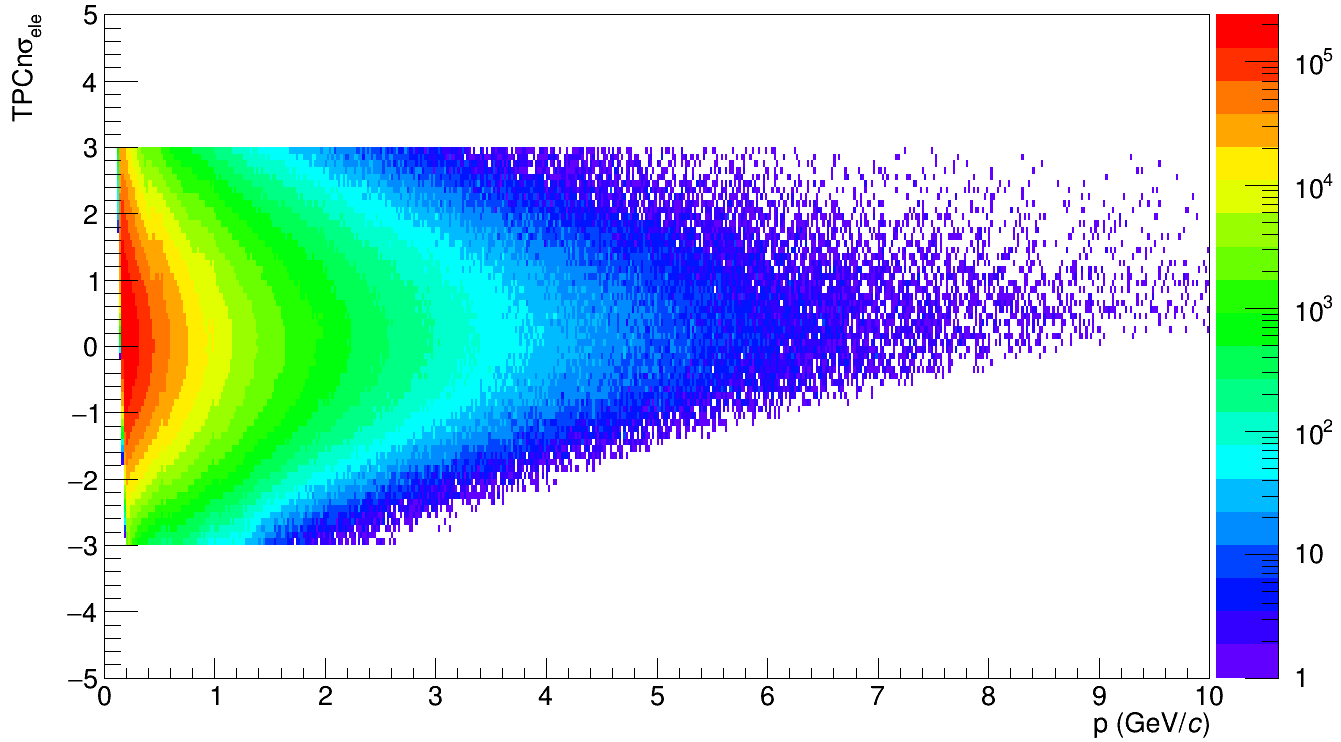
\includegraphics[width=0.98\linewidth]{Figures/V0cuts/tpcnsigmaeleneg.png}
\caption{$n\sigma_e$ versus $p$ plot for the assumption of an electron}
\label{fig:V0tpcele}
\end{subfigure} \hspace{0.1cm}
\begin{subfigure}[t]{.5\linewidth}
\centering
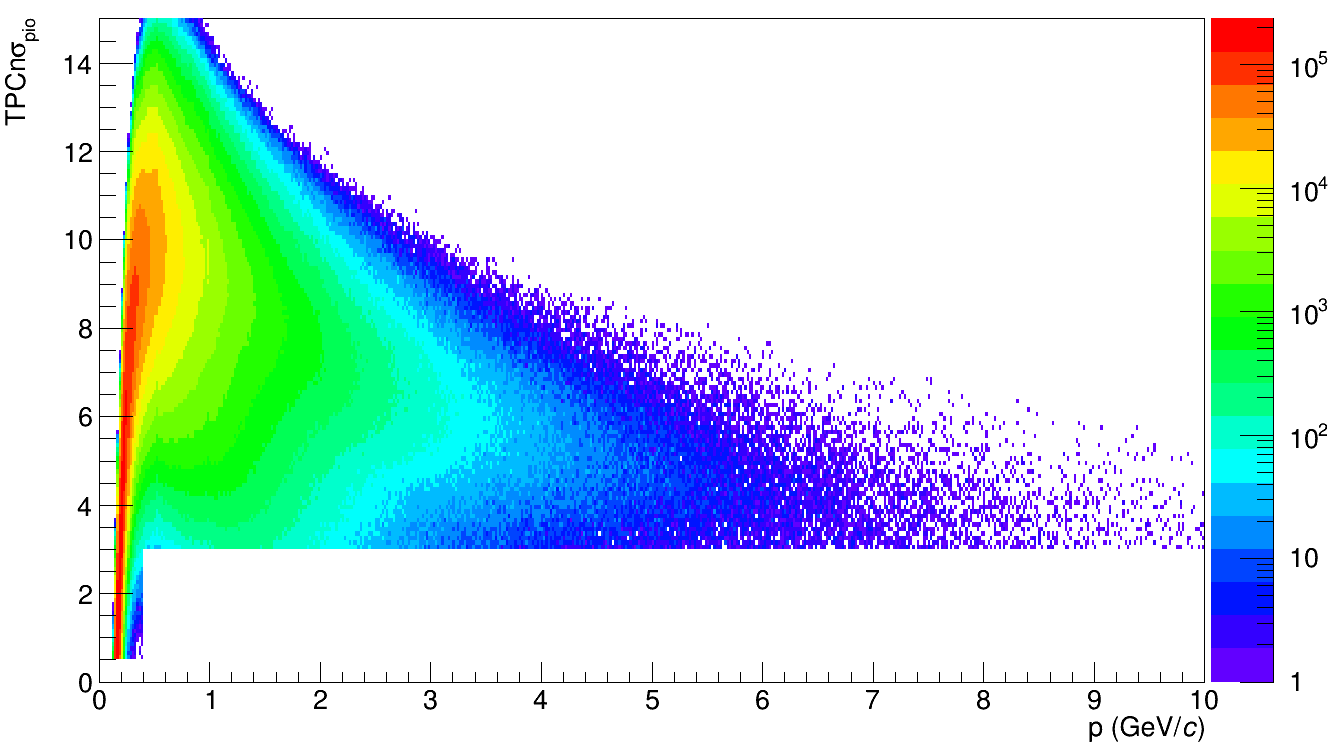
\includegraphics[width=0.98\linewidth]{Figures/V0cuts/tpcnsigmapioneg.png}
\caption{$n\sigma_{\pi}$ versus $p$ plot for the assumption of a pion}
\label{fig:V0tpcpio}
\end{subfigure}
\caption{The specific energy loss of the particles in the TPC expressed in terms of the $n\sigma$ discrimination variable plotted against the particle momentum, here only shown for the negative particles; the colour scale shows the number of counts}
\label{fig:V0tpc}
\end{figure}

\textbf{V$^0$ cuts} \\


quote and discuss cuts (see bachelor thesis for discussion which is basically the same, also add the other cuts which where not used and discuss why they were not used) \\  

V0 cuts
show helix cut, but no cut on helix radius

\begin{sidewaysfigure}[p!]
\centering
\begin{subfigure}[h]{.4\linewidth}
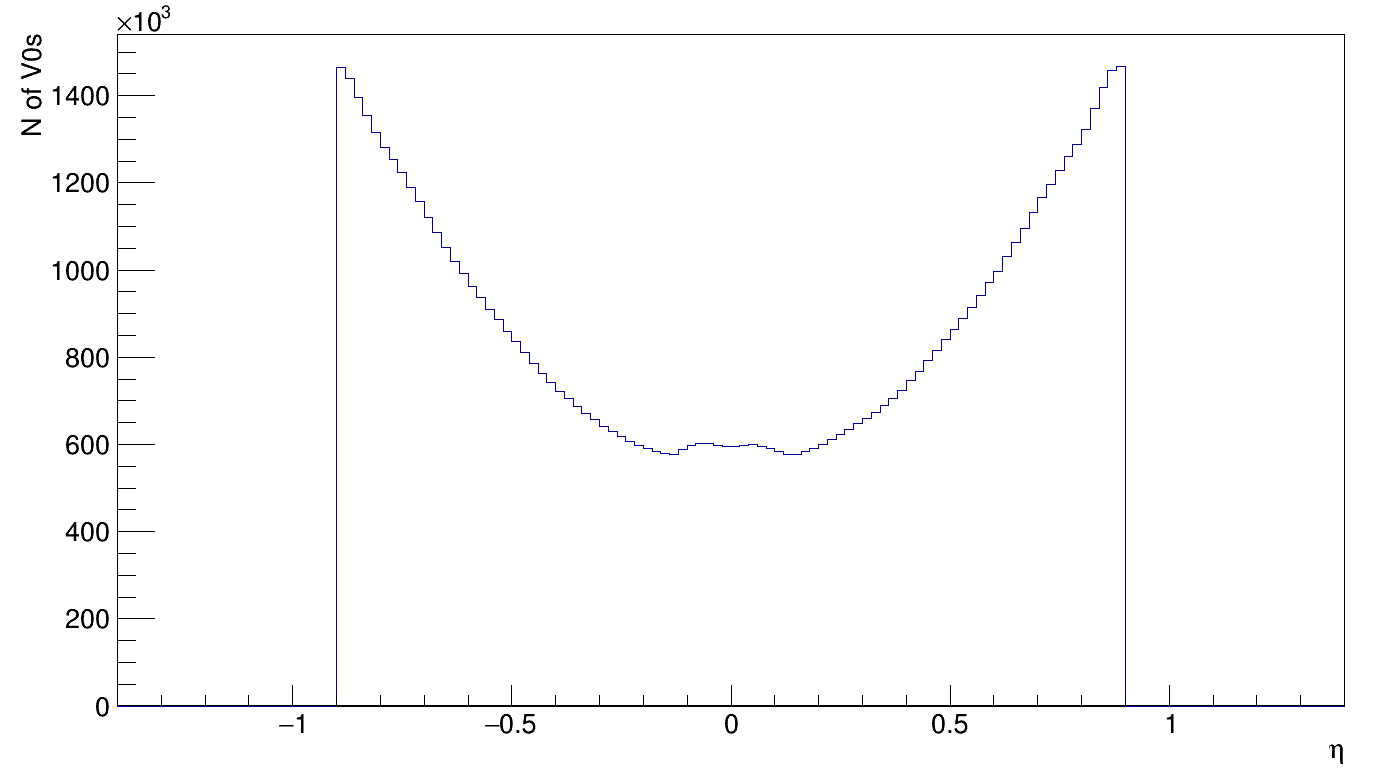
\includegraphics[width=1.0\linewidth]{Figures/V0cuts/V0eta.png}
\caption{Pseudorapidity of the V$^0$ candidate plotted against the number of counts}
\label{fig:V0eta}
\end{subfigure}\hspace{1cm}%
\begin{subfigure}[h]{.4\linewidth}
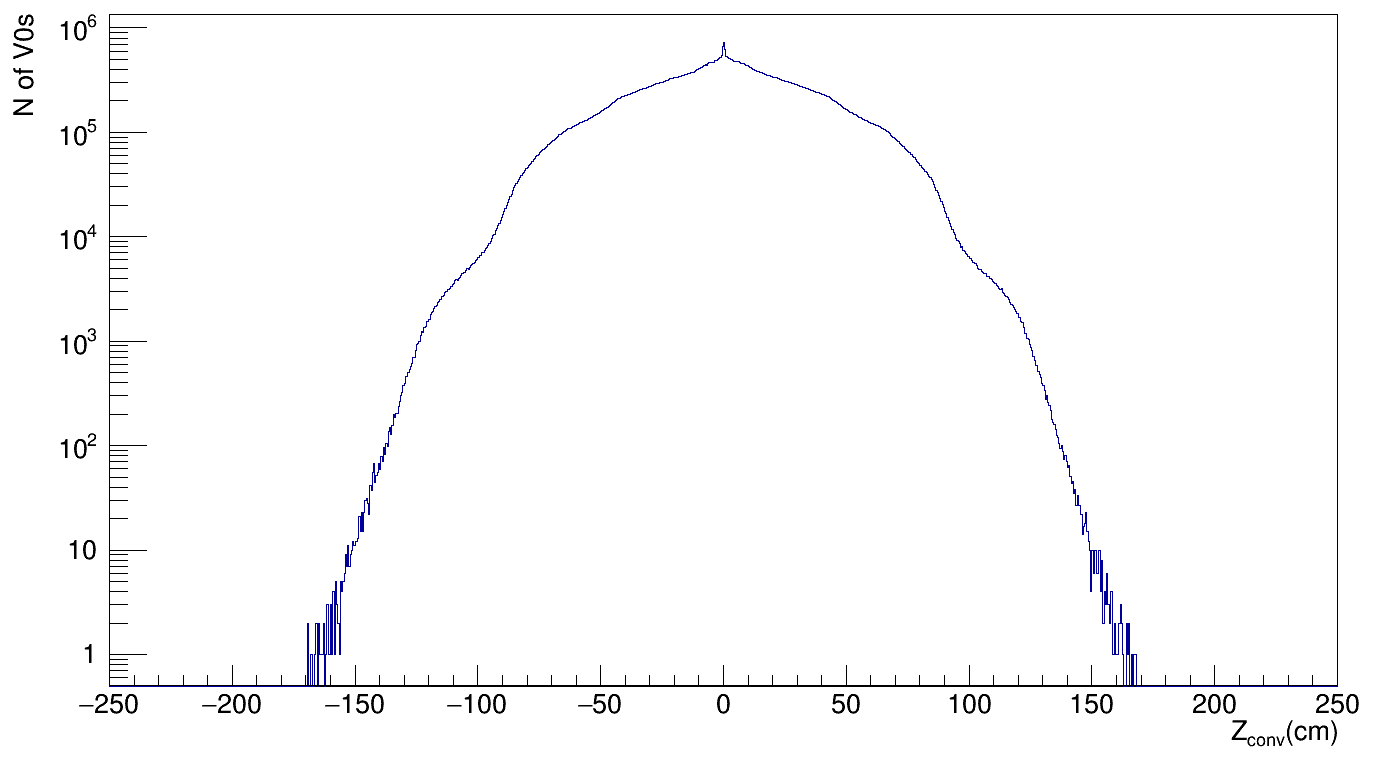
\includegraphics[width=1.0\linewidth]{Figures/V0cuts/V0Z.png}
\caption{$Z$ coordinate of the conversion point plotted against the number of counts}
\label{fig:V0Z}
\end{subfigure}

\vspace{0.7cm}

\begin{subfigure}[h]{.4\linewidth}
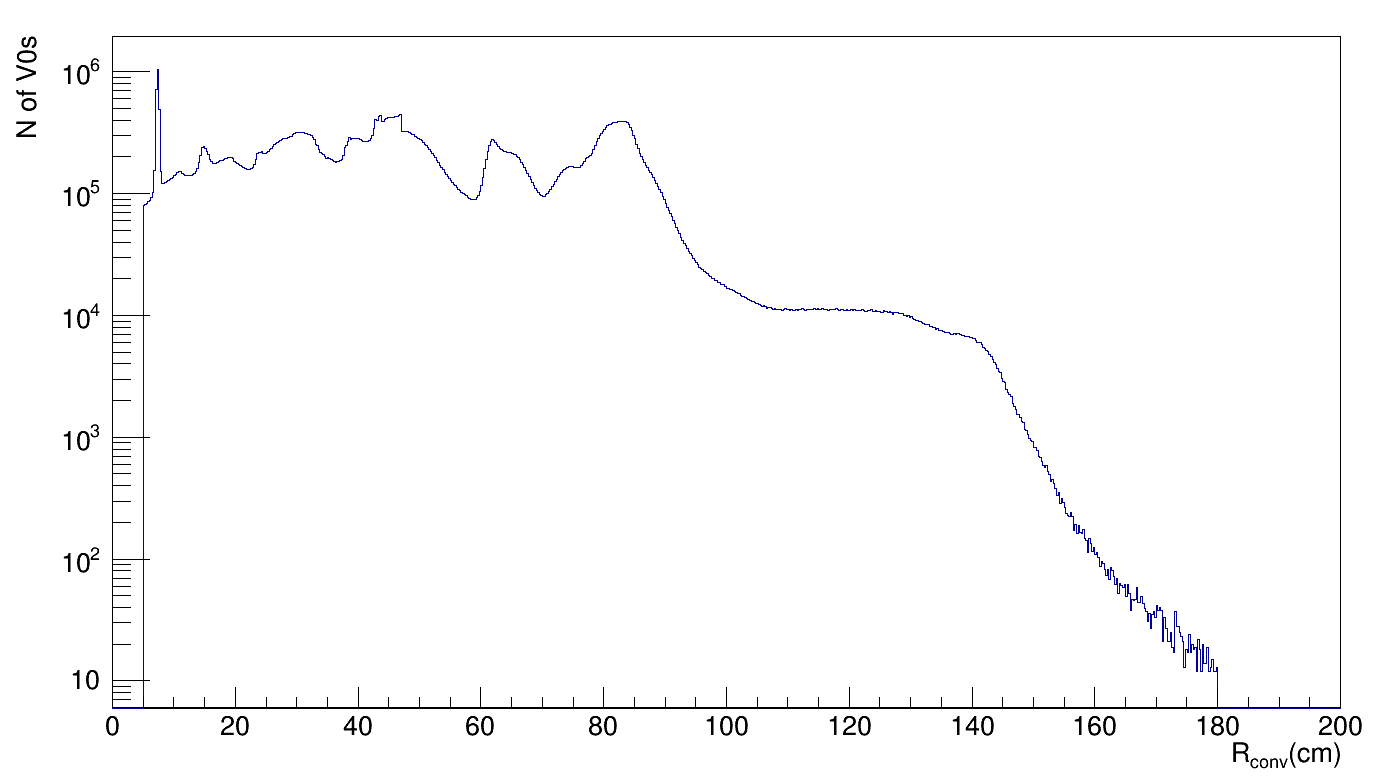
\includegraphics[width=1.0\linewidth]{Figures/V0cuts/V0radius.png}
\caption{\centering{Radius of the conversion point plotted against the number of counts}}
\label{fig:V0R}
\end{subfigure}\hspace{1cm}%
\begin{subfigure}[h]{.4\linewidth}
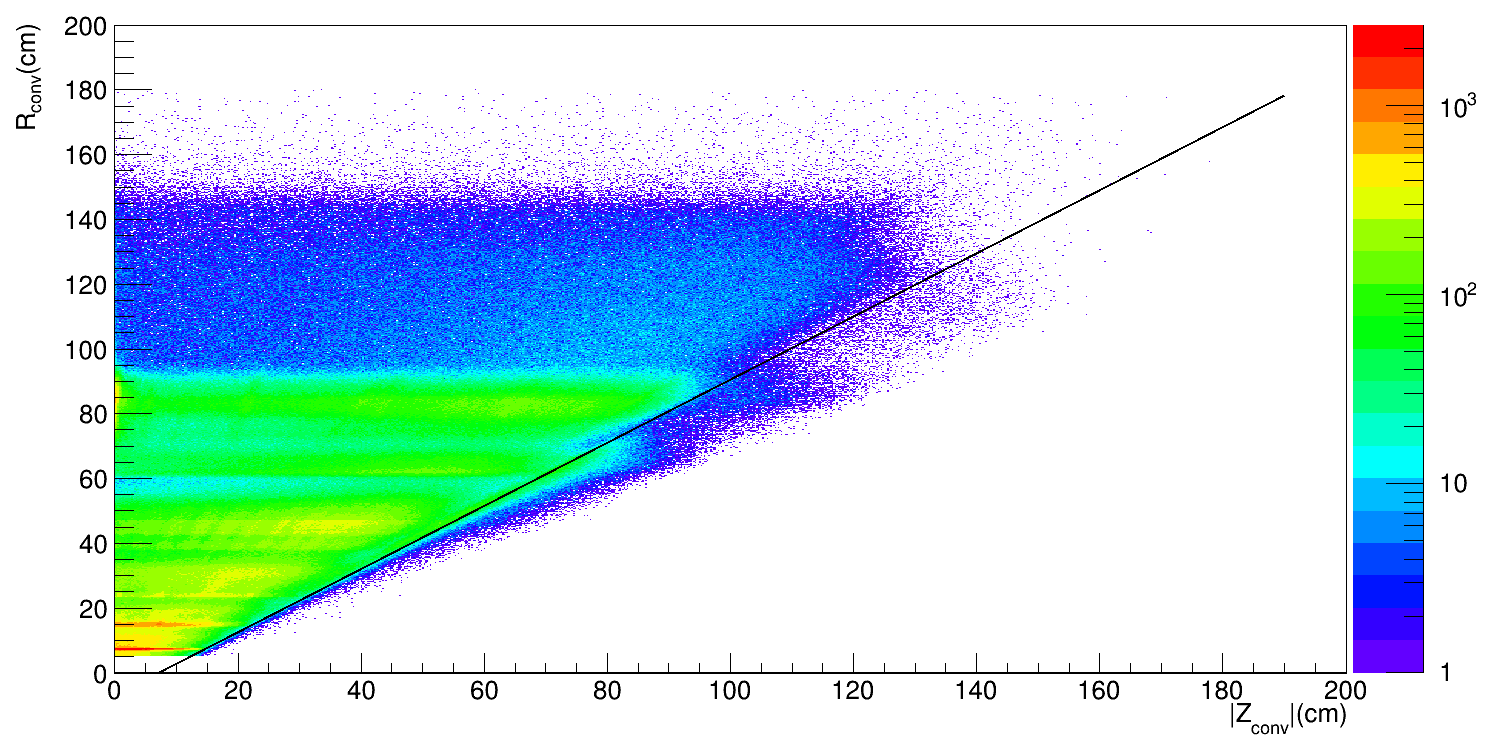
\includegraphics[width=1.0\linewidth]{Figures/V0cuts/V0RvsZwlinecut.png}
\caption{$Z$ coordinate of the conversion point plotted against the radius of the conversion point; the line shows the line cut defined in table \ref{tab:V0cuts} and the colour scale shows the number of counts}
\label{fig:V0linecut}
\end{subfigure}
\vspace{0.5cm}
\caption{Plots of the geometric V$^0$ cuts as they were used in this analysis}
\label{fig:V0cuts}
\end{sidewaysfigure}
\begin{sidewaysfigure}[p!]
\centering
\begin{subfigure}[h]{.4\linewidth}
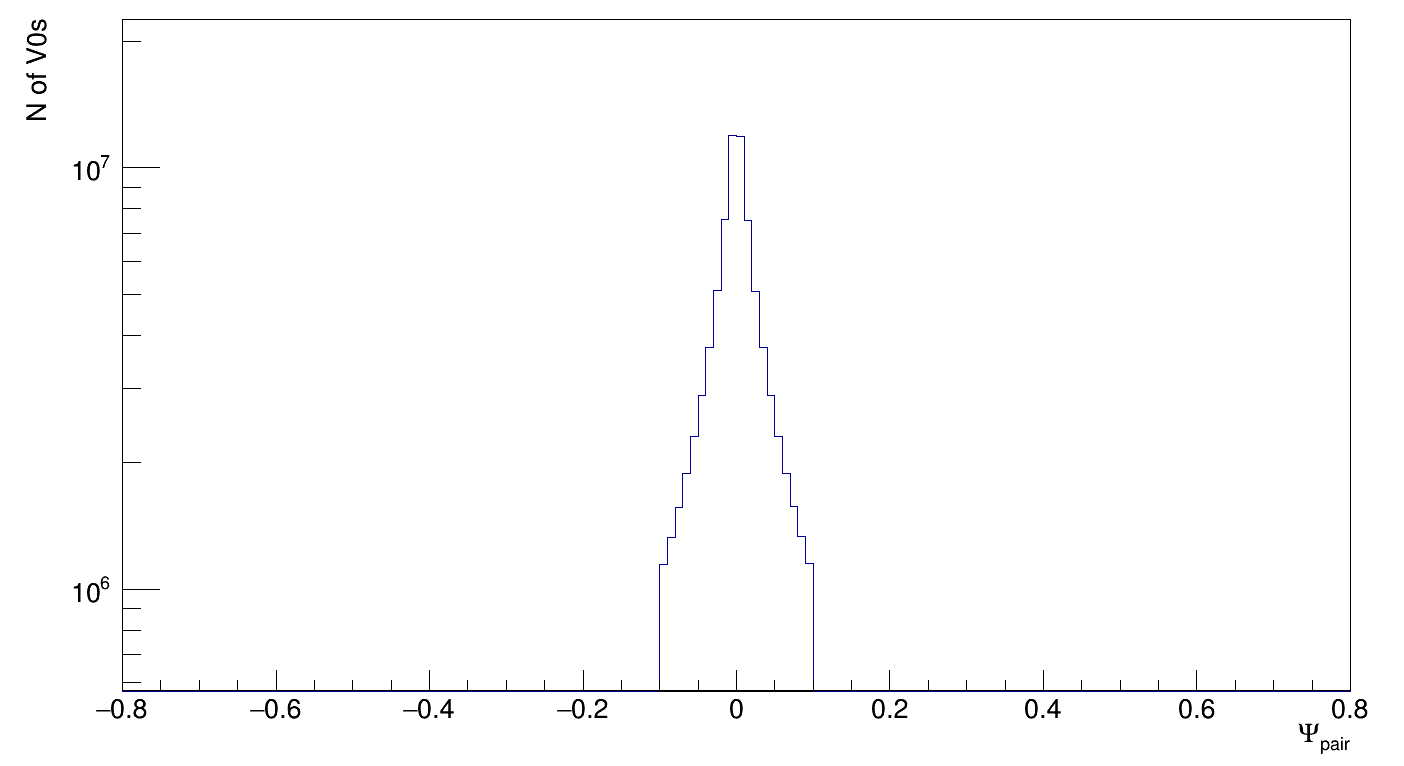
\includegraphics[width=1.0\linewidth]{Figures/V0cuts/V0psipair.png}
\caption{$\Psi_{pair}$ angle of the V$^0$ candidate plotted against the counts}
\label{fig:V0psipair}
\end{subfigure}\hspace{1cm}%
\begin{subfigure}[h]{.4\linewidth}
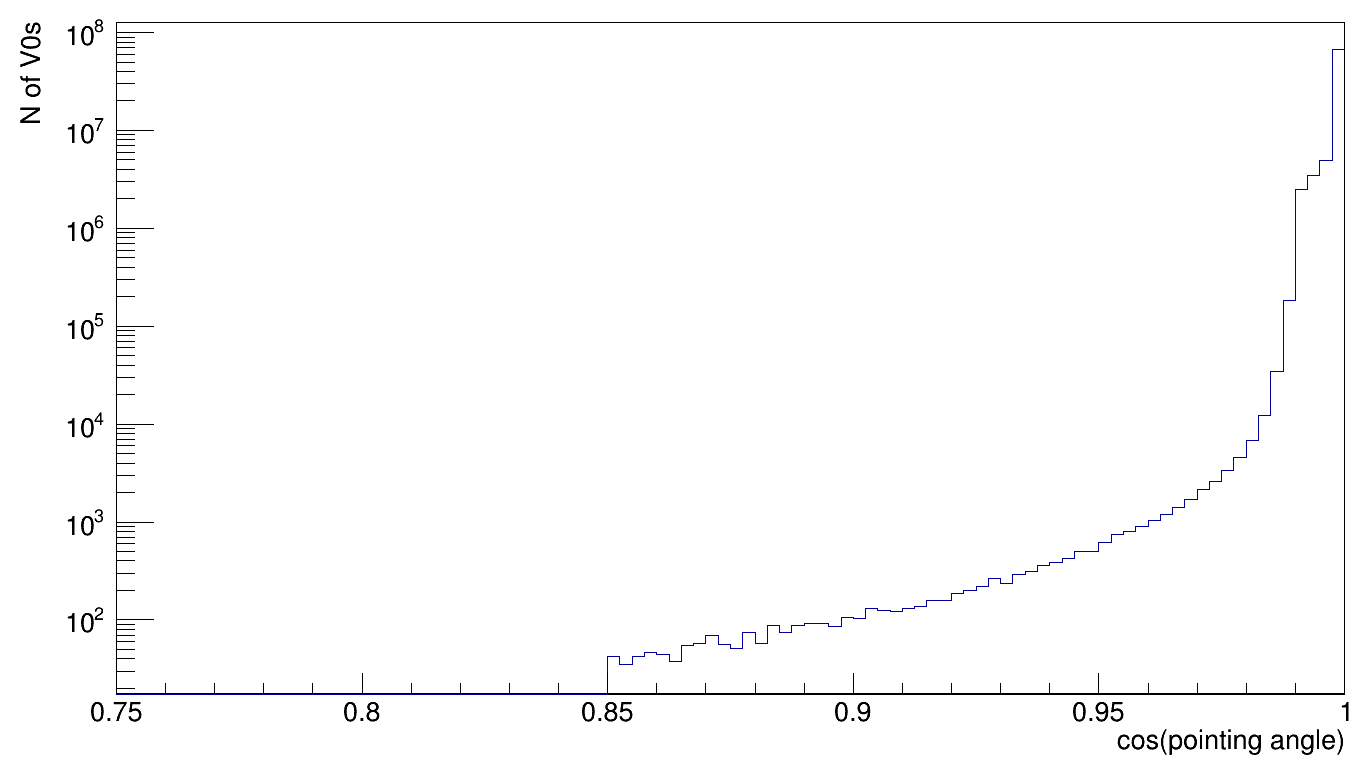
\includegraphics[width=1.0\linewidth]{Figures/V0cuts/V0cospa.png}
\caption{cos(pointing angle) of the legs of the V$^0$ plotted against the counts}
\label{fig:V0cospa}
\end{subfigure}

\vspace{0.7cm}

\begin{subfigure}[h]{.4\linewidth}
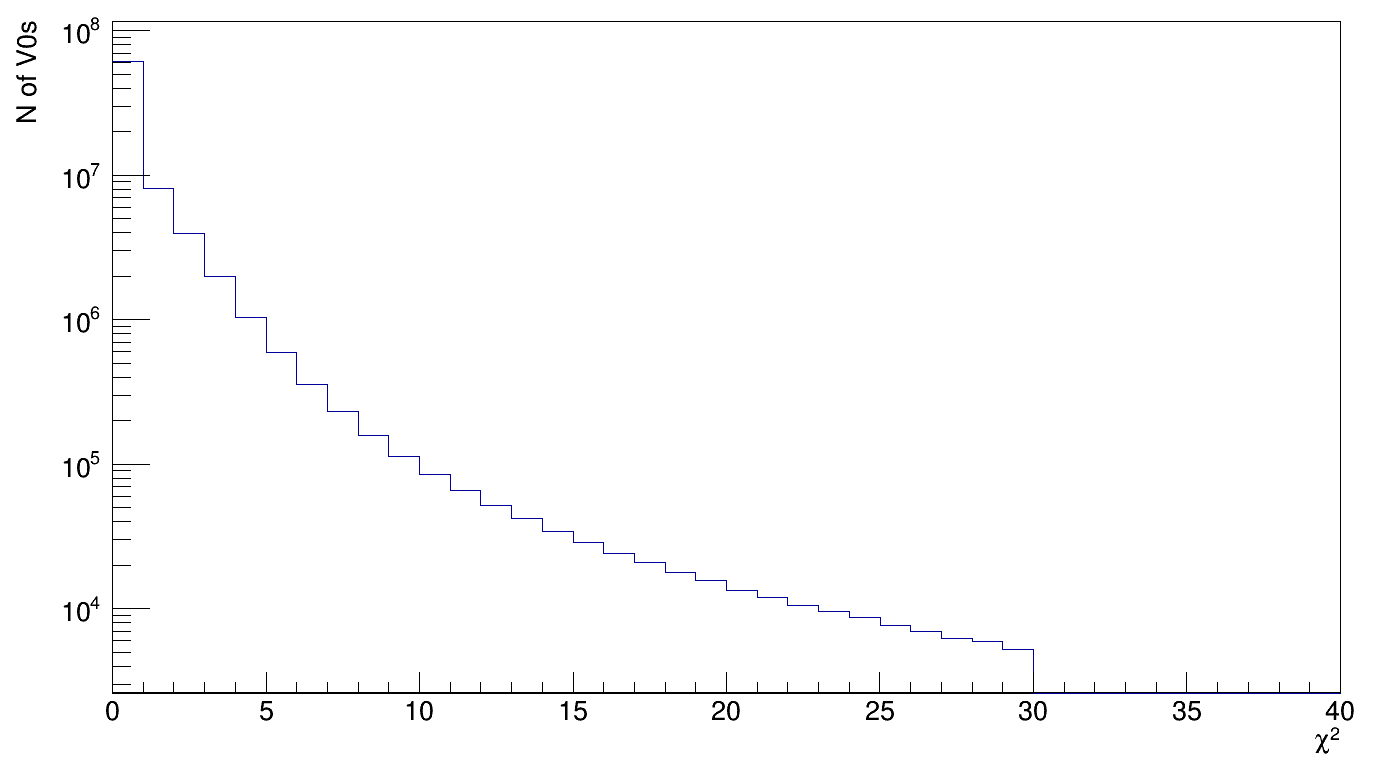
\includegraphics[width=1.0\textwidth]{Figures/V0cuts/V0chi2.png}
\caption{$\chi^2$ of the Kalman filtering method of tracks which form the V$^0$ plotted against the counts}
\label{fig:V0chi2}
\end{subfigure}\hspace{1cm}%
\begin{subfigure}[h]{.4\linewidth}
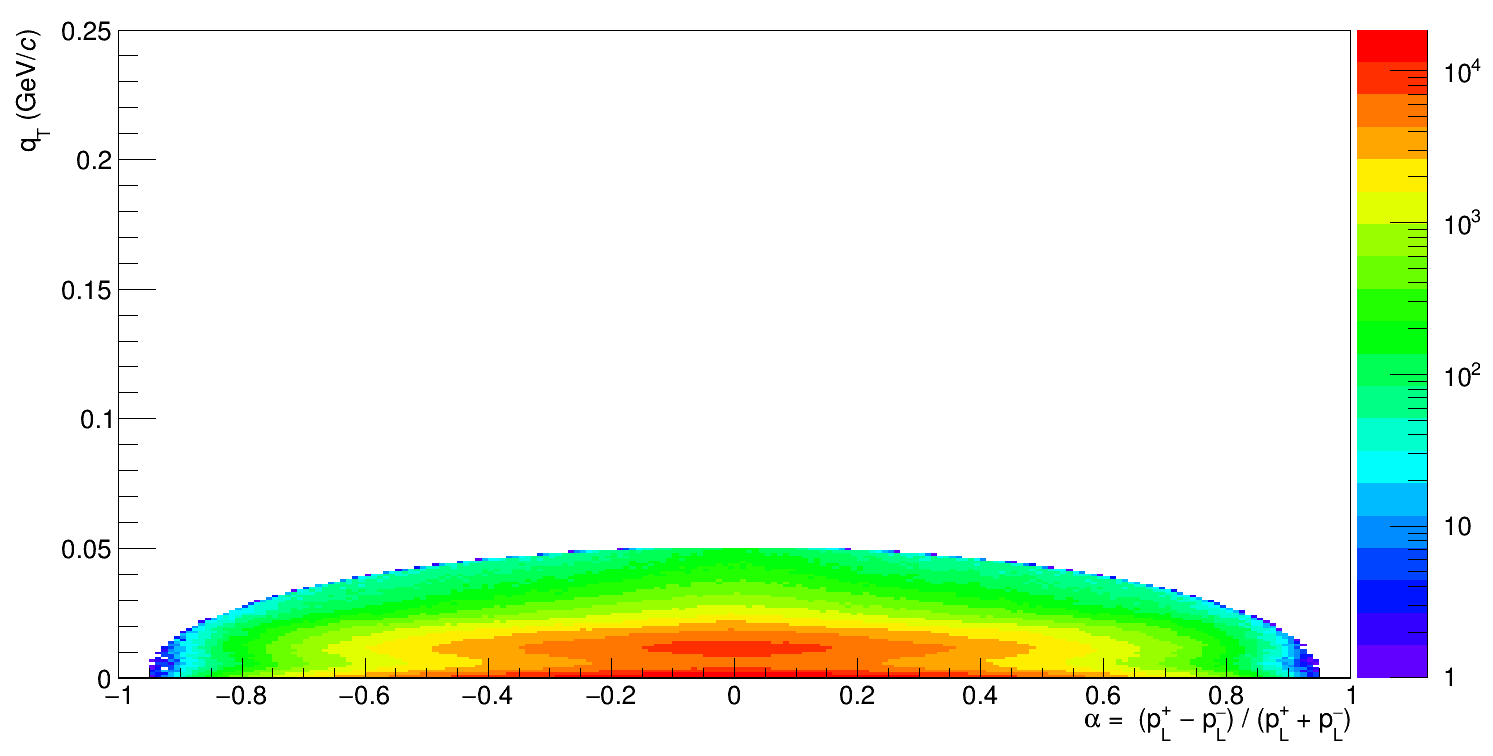
\includegraphics[width=1.0\linewidth]{Figures/V0cuts/armpod.png}
\caption{Armenteros-Podolanski plot with the cut selecting the photons from the V$^0$ candidates}
\label{fig:V0armpod}
\end{subfigure}
\vspace{0.5cm}
\caption{Plots of the further V$^0$ cuts as they were used in this analysis}
\label{fig:V0cuts}
\end{sidewaysfigure} 
blablablablabla








  \renewcommand{\arraystretch}{1.3}
\begin{table}[h]
\centering{
\begin{tabular}{@{} ll @{}}
  \toprule			
  V$^0$ Cut & Cut Range \\ \midrule
  pseudorapidity of CP &  $|\eta_{\text{conv}}| < 0.9$ \\ 
  $Z$ coordinate of CP &  $|Z_{\text{conv}}| < 240$ cm \\ 
  radius of CP  &  $5 \ \text{cm} \ < |R_{\text{conv}}| < 180$ cm \\ 
  line cut  &  $R_{\text{conv}} > |Z_{\text{conv}}| \cdot f \left(\eta_{\text{max}} \right) - Z_0 $\\
  & with $Z_0 = 7$ cm and $\eta_{\text{max}} = 0.9$ \\ 
 $\Psi_{\text{pair}}$ angle  &  $|\Psi_{\text{pair}}| < 0.1$ \\ 
 cosine of pointing angle  &  $\text{cos} \left( \text{pointing angle} \right) > 0.85$ \\ 
 $\chi^2$ of Kalman filter  &  $\chi^2 < 30$ \\
 like-sign cut & reject V$^0$s with like-sign charged legs \\
elliptical cut in Armenteros- \qquad \ \ &  $q_T < q_{T,\text{max}} \cdot \sqrt{1- \alpha^2/\alpha_{\text{max}}^2}$ \\ 
 Podolanski plot &  with $q_{T,\text{max}} = 0.05$ GeV/c, $\alpha_{\text{max}} = 0.95$ \\
  \bottomrule
\end{tabular}
}
\caption{V$^0$ cuts used in the analysis; CP $\widehat{=}$ Conversion Point; $f \left(\eta_{\text{max}} \right)$ is defined in equation \ref{slope}}
\label{tab:pi0gammaV0cuts}
\end{table}
\renewcommand{\arraystretch}{1.0}


\subsection{$a_1 \rightarrow \pi^0\pi^{+}\pi^{-}$ analysis}
\subsubsection{Cuts and Event Selection}
quote and discuss cuts

ele track cuts: same as for other analysis
    
    
\renewcommand{\arraystretch}{1.3}
\begin{table}[h]
\centering{
\begin{tabular}{@{} ll @{}}
  \toprule		
  Track Cut \qquad & \qquad Cut Range \\ \midrule
  track $p_T$ \qquad & \qquad $p_T > 0.05$ GeV/c \\ 
  TPC clusters \qquad & \qquad $\frac{N_{\text{TPC-Clusters}}}{N_{\text{findable TPC-Clusters}}} > 0.6$ \\
  require TPC refit \qquad & \qquad TRUE \\ 
  rejection of tracks with kinks \qquad & \qquad TRUE \\ 
  \midrule
  electron selection \qquad & \qquad $|n\sigma_e| < 3$ \\ \
  pion rejection \qquad & \qquad for $p < 0.4$ GeV/c: $n\sigma_{\pi} < 0.5$ \\
 \qquad & \qquad for $p > 0.4$ GeV/c: $n\sigma_{\pi} < 3$ \\
  \bottomrule 
\end{tabular}
}
\caption{General track and PID cuts for the electron candidates from photon conversions from the $\pi^0 \rightarrow \gamma\gamma$ decay}
\label{tab:3pielecuts}
\end{table}
  \renewcommand{\arraystretch}{1.0}
  

cuts on charged pions:


  856   esdTrackCuts->SetRequireSigmaToVertex(kFALSE);



\renewcommand{\arraystretch}{1.3}
\begin{table}[h]
\centering{
\begin{tabular}{@{} ll @{}}
  \toprule		
  Track Cut \qquad & \qquad Cut Range \\ \midrule
  track $p_T$ \qquad & \qquad $p_T > 0.05$ GeV/c \\ 
  track pseudorapidity \qquad & \qquad $|\eta| < 0.8$ \\ 
  TPC clusters \qquad & \qquad $\frac{N_{\text{TPC-Clusters}}}{N_{\text{findable TPC-Clusters}}} > 0.8$ \\
  crossed TPC rows \qquad & \qquad $N_{\mathrm{crossed \ rows}} > 70 $ \\
  TPC cluster $\chi^2$ \qquad & \qquad $\frac{\chi^2}{N_{\mathrm{clusters}}} < 4 $ \\
  require TPC refit \qquad & \qquad TRUE \\ 
  require ITS refit \qquad & \qquad TRUE \\ 
  DCA to vertex $p_T$ dependence $\chi^2$ \qquad & \qquad $ 0.0105+\frac{0.0350}{p_T^{1.1}}$ \\
  DCA z-coord. to vertex $\chi^2$ \qquad & \qquad $ z_{DCA} < 2$ cm \\
  ITS cluster $\chi^2$ \qquad & \qquad $\frac{\chi^2}{N_{\mathrm{clusters}}} < 36 $ \\
  $\chi^2$ constrained vs global track \qquad & \qquad $\chi^2 < 36$ \\ 
  rejection of tracks with kinks \qquad & \qquad TRUE \\ 
  require sigma to vertex \qquad & \qquad FALSE \\ 
  \midrule
  pion selection \qquad & \qquad $|n\sigma_{\pi,TPC}| < 3$ \\ \
 \qquad & \qquad $|n\sigma_{\pi,TOF}| < 3$ \\
  \bottomrule 
\end{tabular}
}
\caption{General track and PID cuts for the pions from the $a_1 \rightarrow \pi^0\pi^{+}\pi^{-}$ decay}
\label{tab:3pipiocuts}
\end{table}
  \renewcommand{\arraystretch}{1.0}


\subsection{MC production}
